% The pictures drawed in https://www.draw.io/

\documentclass[xcolor=table]{beamer}
% theme
\mode<presentation>
{
	%\usetheme{Warsaw}
	\usetheme{boxes}
	%\useoutertheme{infolines} 
	\setbeamercovered{transparent}
  \usecolortheme{dolphin}
} 

\usepackage[english]{babel}
\usepackage{CJKutf8}
\usepackage{listings}
\usepackage{multirow}
\usepackage{textpos}
\usepackage{xcolor}
\usepackage{animate}
\usepackage[table]{xcolor}

\setbeamertemplate{footline}[frame number]
\setbeamertemplate{section in toc}{\inserttocsectionnumber.~\inserttocsection}

\setbeamercolor*{block title}{fg=black, bg= blue!10}
\setbeamercolor*{block body}{fg= blue, bg= blue!5}
\definecolor{dgreen}{rgb}{0.,0.6,0.}

\begin{document}
\begin{CJK}{UTF8}{gkai}

% title	
\title[刘绍辉]{小米HBase实践}
\author{刘绍辉}
%{\\ liushaohui@xiaomi.com \\ 微博: lshmouse}
\institute{小米云存储组}
\date{China Hadoop Summit 2013}


\begin{frame}[plain]
  \titlepage
\end{frame}

% xiaomi logo
\addtobeamertemplate{frametitle}{}{%
	\begin{textblock*}{200mm}(0.8\textwidth,-0.6cm)
		
\includegraphics[height=1cm]{xiaomi.png}
	\end{textblock*}}

% outlines
\begin{frame}{提纲}
  \tableofcontents[hideallsubsections]
\end{frame}

\AtBeginSection{
	\begin{frame}{提纲}
	  \tableofcontents[currentsection,hideallsubsections]
  \end{frame}
}

\section{HBase简介}
\begin{frame}{HBase是什么?}
\begin{itemize}
	\item \textcolor{dgreen}{Google Bigtable系统的开源实现}
	\item	分布式的,可扩展的,一致性的,半结构化数据存储系统
	\item \textcolor{blue}{稀疏的, 一致性的,分布式的, 多维有序的映射表} 
\end{itemize}
\end{frame}

\begin{frame}{数据模型}
\begin{columns}
	\begin{column}{0.4\textwidth}
		\begin{itemize}
			\item 表
			\item 行
			\item 列簇
			\item 列
			\item 版本(时间戳)
		\end{itemize}
	\end{column}
	\begin{column}{0.6\textwidth}
		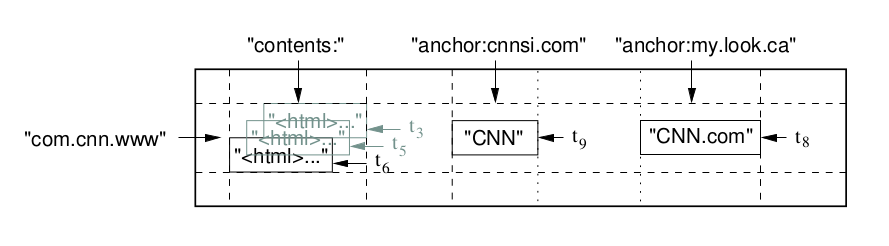
\includegraphics[width=\textwidth, height=4cm]{hbase-data-model.png}
	\end{column}
\end{columns}
	\bigskip
	多维映射表:\\ 
	(行key, 列簇, 列, 版本) $\rightarrow$ 值
\end{frame}

\begin{frame}{逻辑架构}
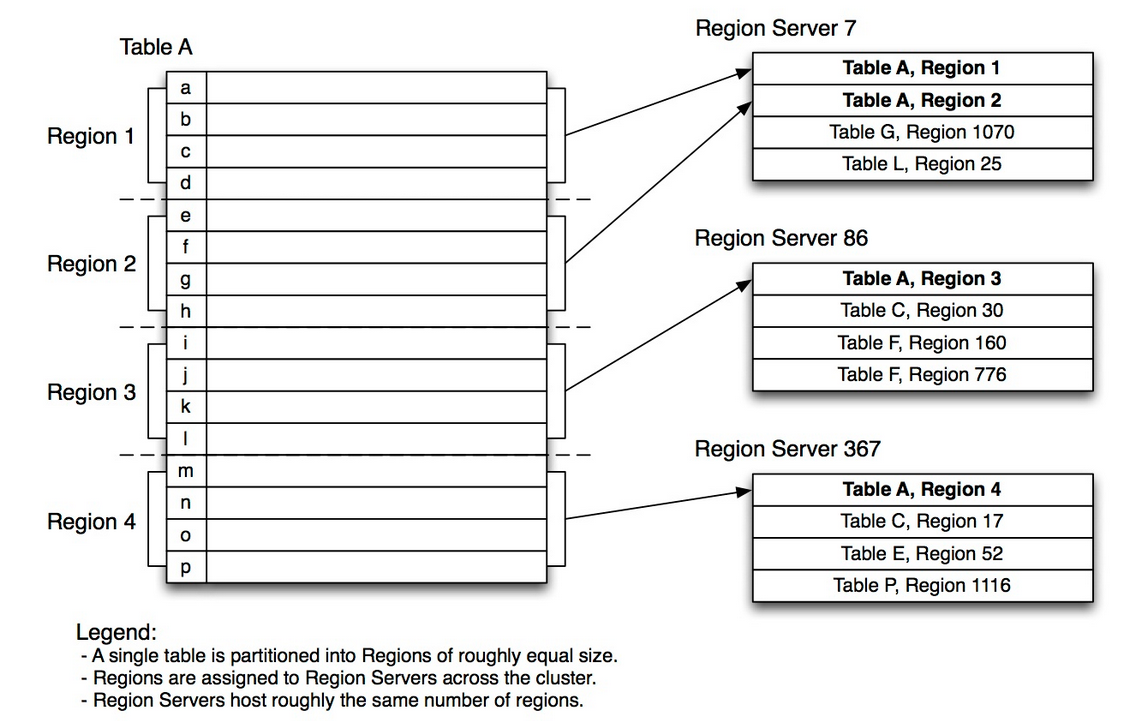
\includegraphics[width=\textwidth, height=6cm]{logical-arch.png} \\
参考: http://www.slideshare.net/xefyr/h-base-for-architectspptx
\end{frame}

\begin{frame}{系统架构}
HMaster负责控制流\\
HRegionServer负责数据流\\
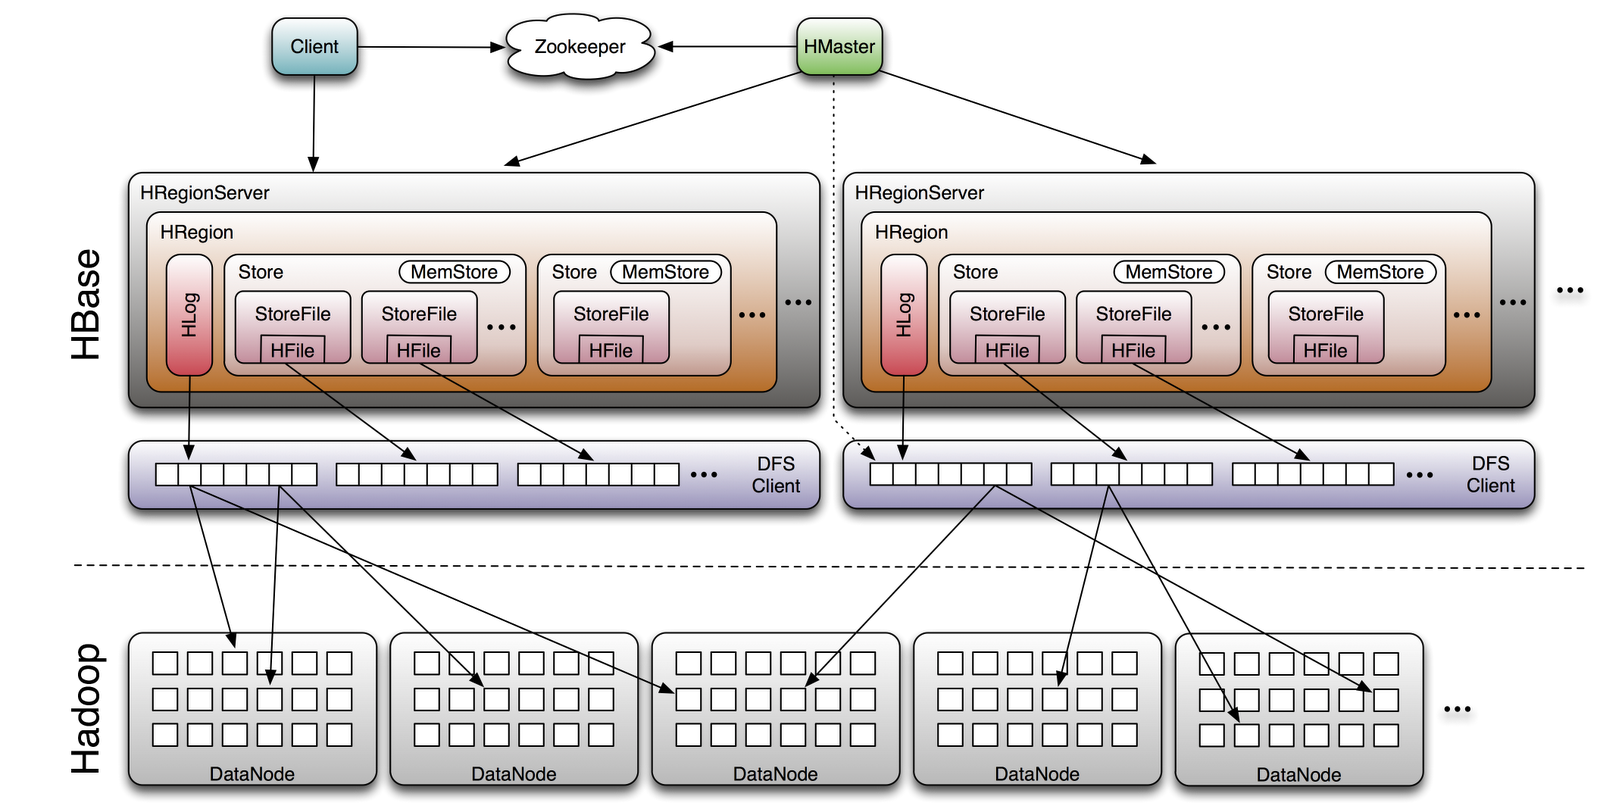
\includegraphics[width=\textwidth, height=6cm]{hbase-arch.png}
\end{frame}

%\begin{frame}{HBase优势}
%	\begin{itemize}
%		\item 水平扩展能力
%		\item 写性能好
%		\item Schema设计灵活
%		\item HBase社区和Hadoop生态系统
%	\end{itemize}
% \end{frame}

\section{HBase在小米的使用}
\subsection{支持的业务}
\begin{frame}{\subsecname}
\begin{columns}
	\begin{column}{0.55\textwidth}
		\begin{itemize}
			\item 米聊消息全存储
			\item MiCloud: 短信, 通话记录同步
			\item 小米Push服务
			\item 其他一些离线分析业务
		\end{itemize}
	\end{column}
	\begin{column}{0.45\textwidth}
		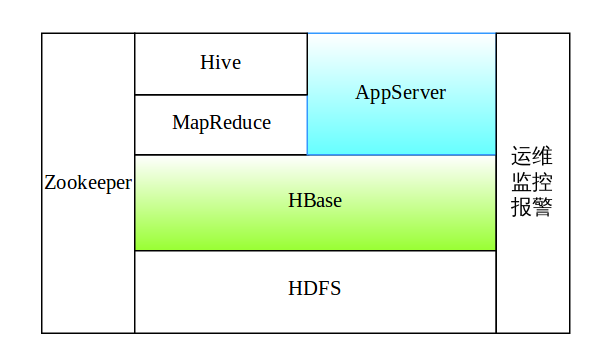
\includegraphics[width=\textwidth, height=4cm]{stack.png}
	\end{column}
\end{columns}
\end{frame}

\subsection{典型的HBase集群}
\begin{frame}{\subsecname}
配置 \\
\bigskip
\begin{tabular}{|c|c|c|c|c|}
	\rowcolor{gray!50}
	\hline
	 节点类型 & 数量		& CPU  & Memory & Disk \\
	\hline
	控制节点 & 3 - 5	& 16核 & 64G    & 6 * 600G SAS, RAID10\\
	\hline
	数据节点 & 5 - N	& 16核 & 64G    & 12 * 2T SATA/SAS \\
	\hline
\end{tabular}  
\end{frame}

\begin{frame}{\subsecname}
\begin{itemize}
\item 控制节点:ZooKeeper, NameNode/ZKFC/JournalNode, HMaster
\item 数据节点: DataNode, RegionServer
\end{itemize}
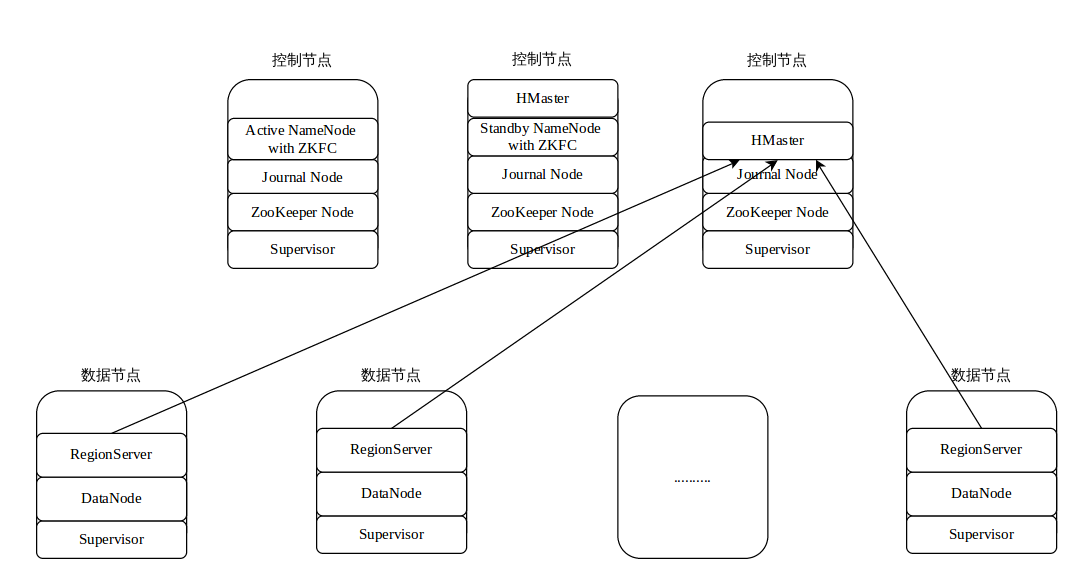
\includegraphics[width=\textwidth, height=6cm]{hbase-init.png}
\end{frame}

\subsection{Minos:自动化部署}
\begin{frame}{\subsecname}
	命令行工具
	\begin{itemize}
	\item 初始化: deploy.py install/bootstrap hbase bjsrv-test
	\item 启/停: deploy.py start/stop hbase bjsrv-test	
	\item 展示: deploy.py show hbase bjsrv-test	
	\item 升级: deploy.py restart/rolling\_update hbase bjsrv-test	
	\item 删除: deploy.py cleanup hbase bjsrv-test	
	\end{itemize}
	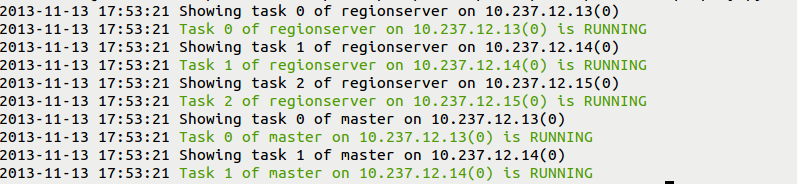
\includegraphics[width=\textwidth, height=3cm]{deploy-show.png}
\end{frame}

\subsection{Minos:监控和报警}
\begin{frame}{\subsecname}
	Dashboard
	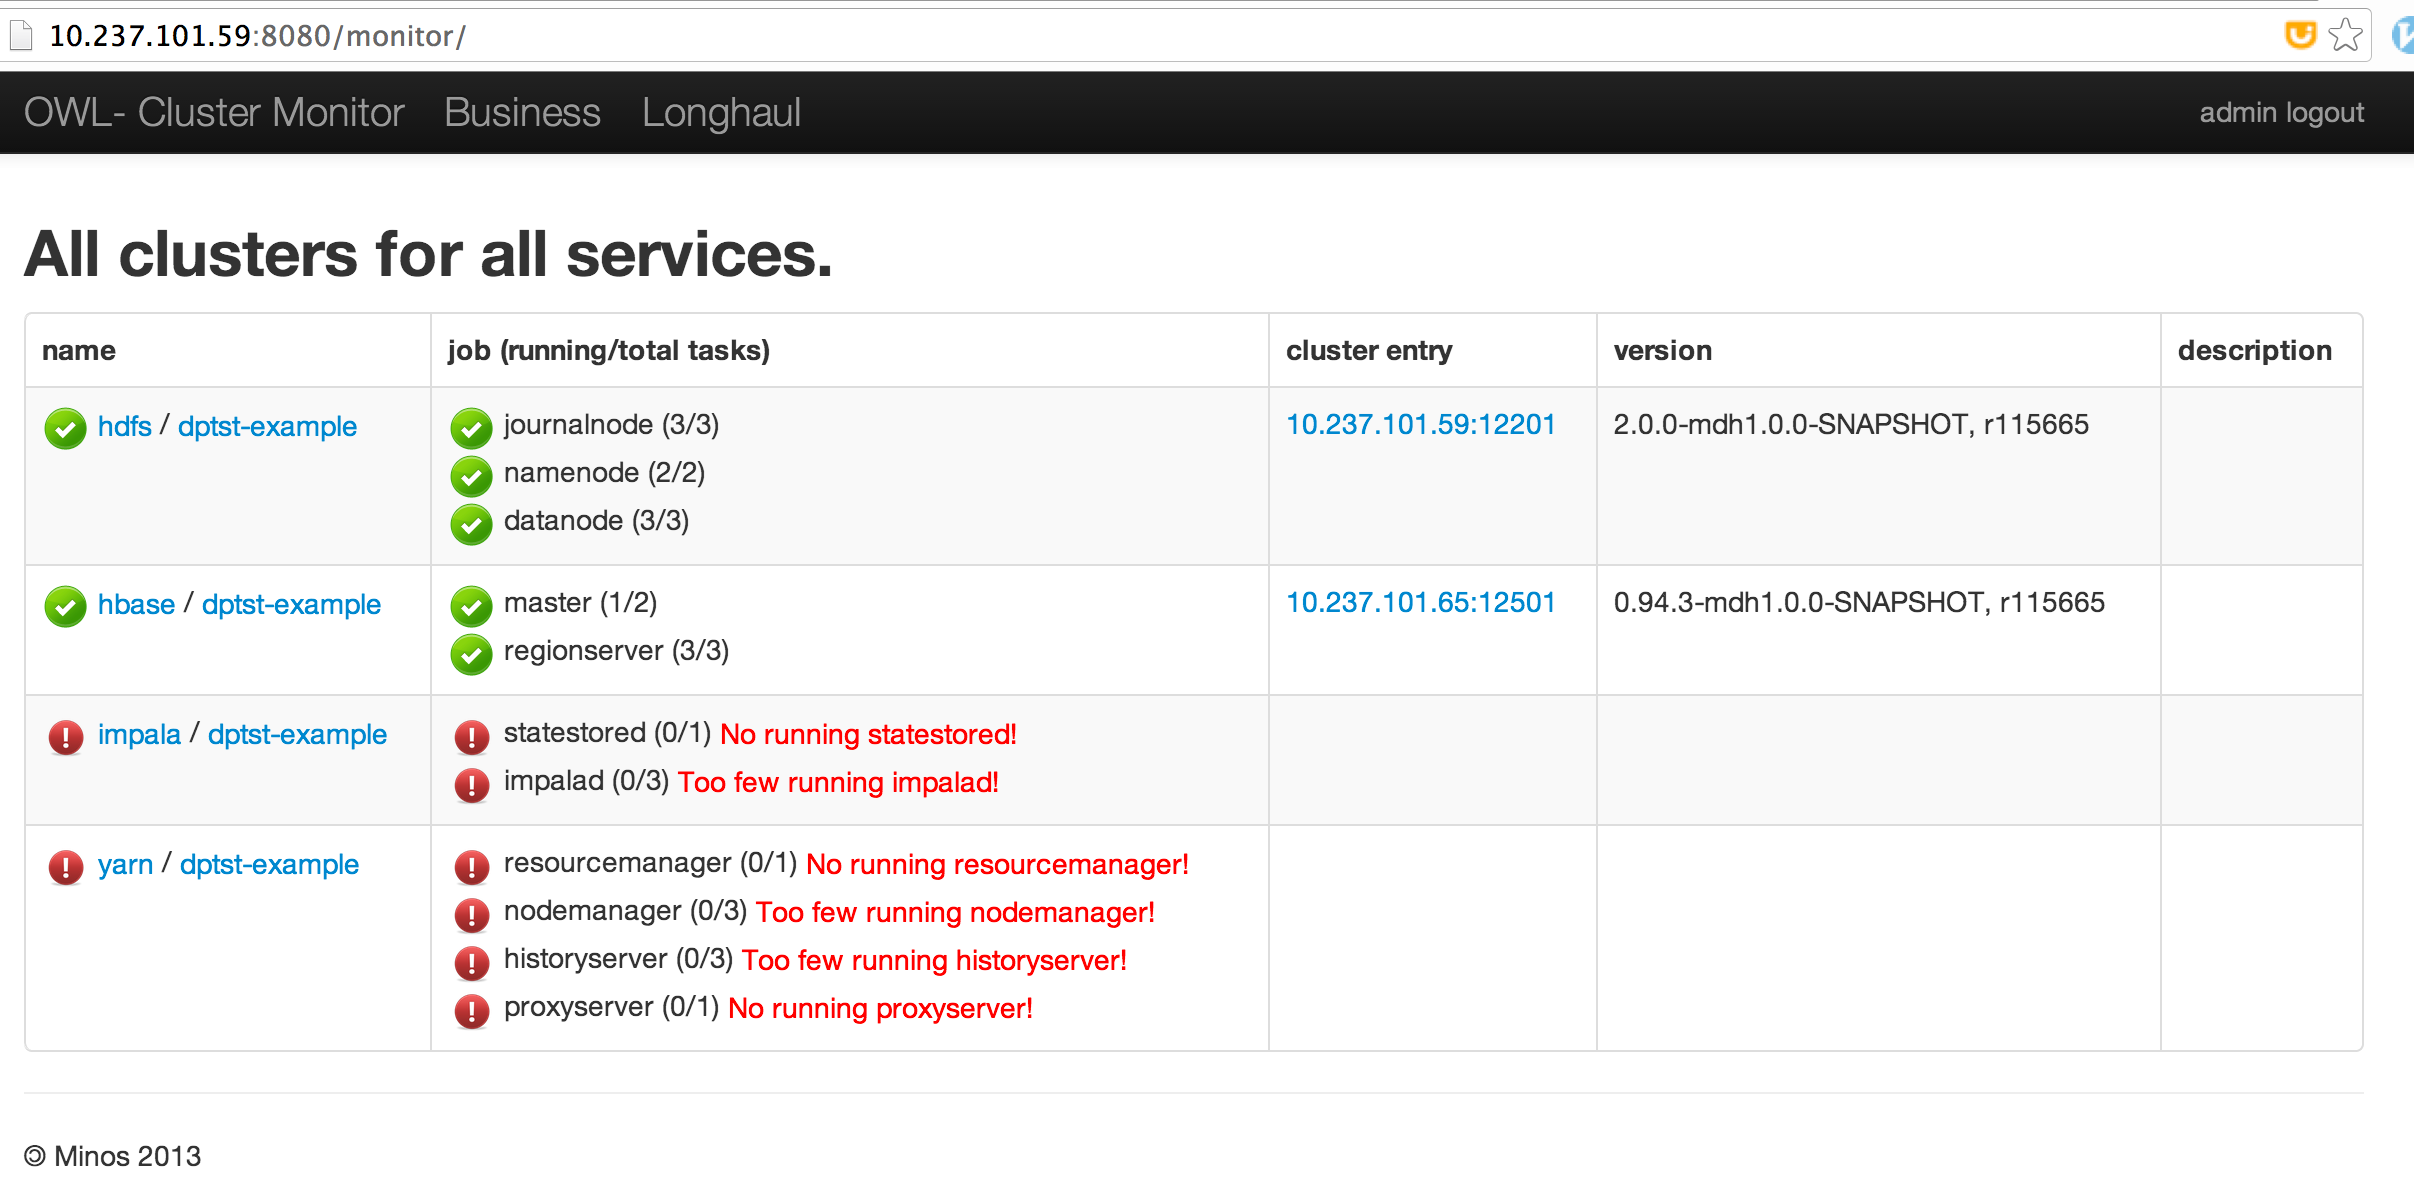
\includegraphics[width=\textwidth, height=7cm]{owl-1.png}
\end{frame}

\begin{frame}{\subsecname}
	Dashboard
	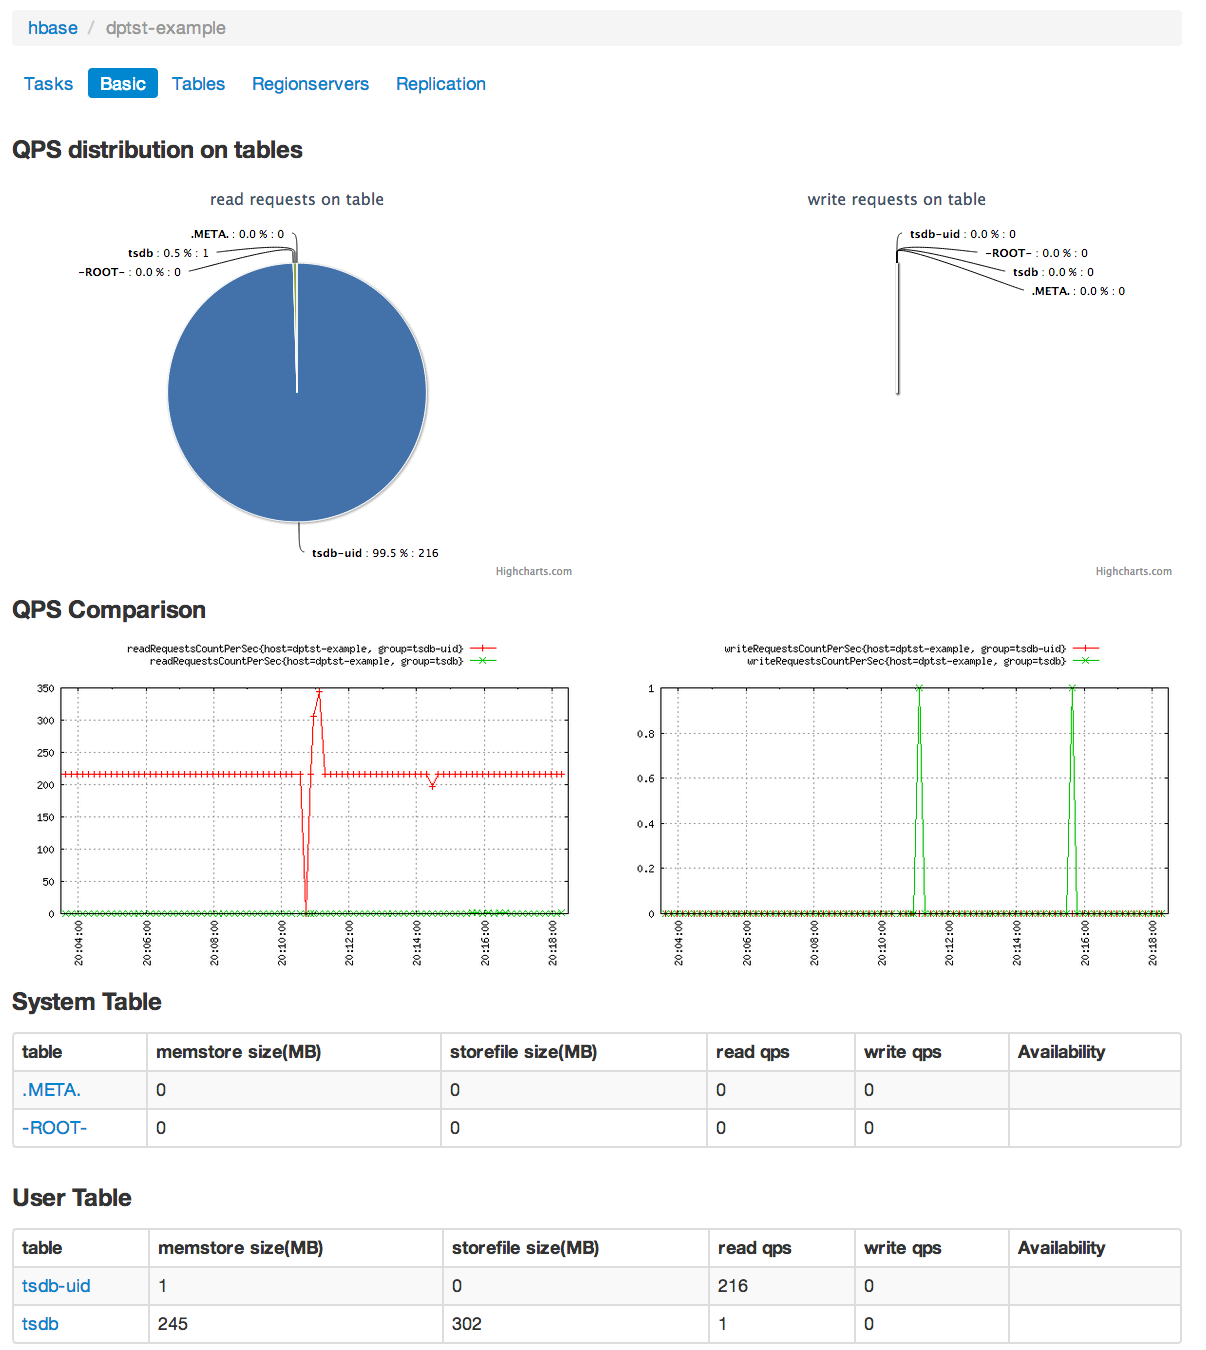
\includegraphics[width=\textwidth, height=7cm]{owl-2.png}
\end{frame}

\begin{frame}{\subsecname}
	性能指标: 分类展示 \\
	基于OpenTSDB: http://opentsdb.net/
	% TODO: 找一个有实际数据的
	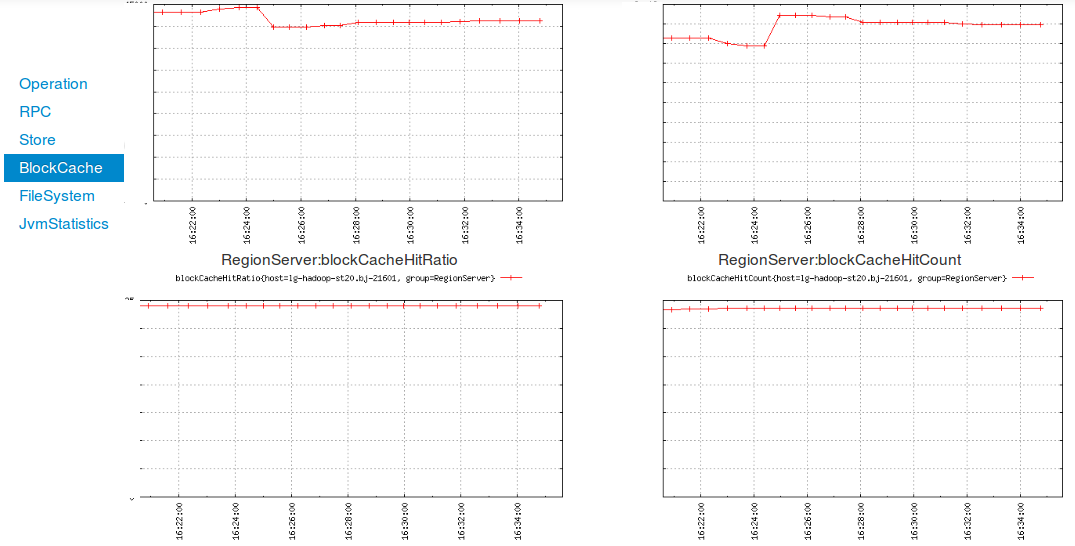
\includegraphics[width=\textwidth, height=7cm]{metrics.png}
\end{frame}

\begin{frame}{Minos}
	\center	开源 https://github.com/xiaomi/Minos \\
	\center{
\includegraphics[width=0.4\textwidth, height=2cm]{minos.png}}

\end{frame}

\subsection{最佳实践}

\begin{frame}{\subsecname}
	HBase Client 封装 \\
	\begin{columns}
	\begin{column}{0.4\textwidth}
		\begin{itemize}
		\item 线程安全
		\item 自动添加性能指标
		\item 跨表、跨集群对用户透明
		\item 动态更新客户端配置
		\end{itemize}
	\end{column}
	\begin{column}{0.6\textwidth}
	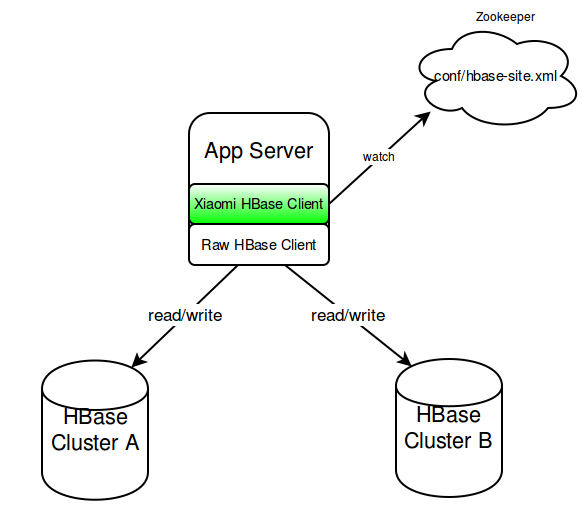
\includegraphics[width=\textwidth, height=6cm]{hbase-client.png}
	\end{column}
\end{columns}

\end{frame}

\begin{frame}{\subsecname}
	跨机房:双主复制 \\
	\begin{columns}
	\begin{column}{0.5\textwidth}
		\begin{itemize}
			\item 中途添加一个复制 \\
				\small add\_peer + CopyTable
	  	\item 复制数据一致性验证 \\
				\small VerifyReplication
		\end{itemize}
	\end{column}
	\begin{column}{0.5\textwidth}
	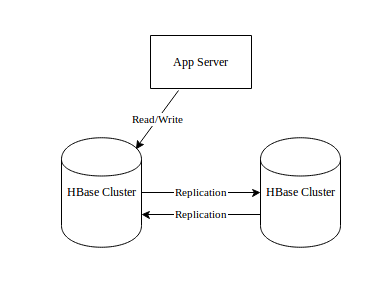
\includegraphics[width=\textwidth, height=4cm]{master-master.png}
	\end{column}
\end{columns}
\end{frame}

\begin{frame}{\subsecname}
	主备集群自动切换
	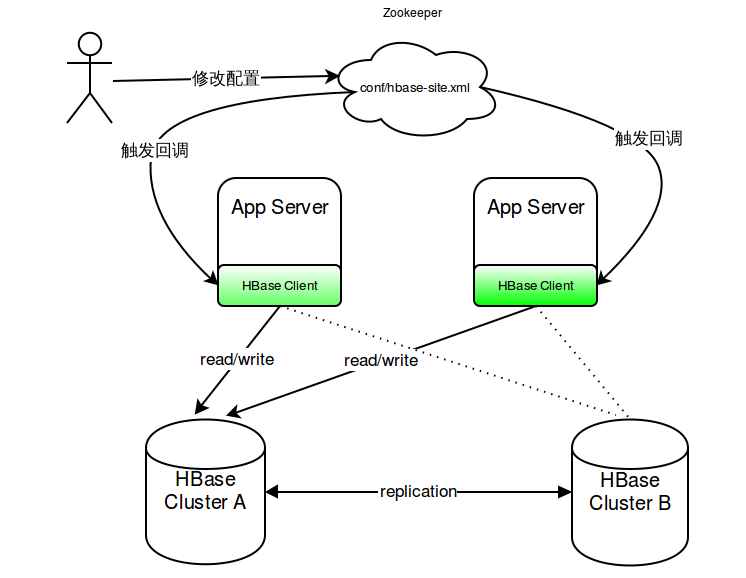
\includegraphics[width=\textwidth, height=6cm]{cluster-switch.png}
\end{frame}

\begin{frame}{最佳实践}
\begin{itemize}
\item 平滑升级 \\
	\small 基于move region脚本, 减少不可用时间
\item Full GC \\
	\small 每天低峰期触发Full GC: jmap -histo:live \$pid
\item Compaction \\
	\small hbase.offpeak.start/end.hour
\item Shortcircuit Read \\
	\small dfs.client.read.shortcircuit
\item 安全 \\ 
	\small Kerberos + HBase ACL
\end{itemize}
\end{frame}

\section{小米开发的重要特性}

\subsection{反向scan}
% 反向scan, 
\begin{frame}{\subsecname}
	正向scan的基本过程 \\
	eg: scan $[r1, r3]$
	\begin{columns}
		\begin{column}{0.5\textwidth}
			\begin{enumerate}
				\item<1-> 顺序读取当前行数据后, 自然读到下一行开头
				\item<4-> 选取最小行作当前行的“下一个行”, 重复上述过程
			\end{enumerate}
		\end{column}
		\begin{column}{0.5\textwidth}
			\includegraphics<1>[width=\textwidth, height=5cm]{scan-s1.png}
			\includegraphics<2>[width=\textwidth, height=5cm]{scan-s2.png}
			\includegraphics<3>[width=\textwidth, height=5cm]{scan-s3.png}
			\includegraphics<4>[width=\textwidth, height=5cm]{scan-s4.png}
		\end{column}
	\end{columns}
\end{frame}

\begin{frame}{\subsecname}
	基本过程: 
	\\ eg: 反向scan $[r2, r0]$ \\
	\begin{columns}
		\begin{column}{0.5\textwidth}
			\begin{enumerate}
				\item<2-> 顺序读取完当前行数据后,
				\item<3->	构造当前行的最小kv, 对每个HFile, SeekBefore $\rightarrow$
					获取这个最小kv的上一个kv
				\item<4-> 选取所有kv中最大行作为当前行的“上一个行”, 
					构造并seek到上一个行的最小kv位置
			\end{enumerate}
		\end{column}
		\begin{column}{0.5\textwidth}
			\includegraphics<1>[width=\textwidth, height=5cm]{rscan-s1.png}
			\includegraphics<2>[width=\textwidth, height=5cm]{rscan-s2.png}
			\includegraphics<3>[width=\textwidth, height=5cm]{rscan-s3.png}
			\includegraphics<4>[width=\textwidth, height=5cm]{rscan-s4.png}
		\end{column}
	\end{columns}
%	反向scan会多一次seekBefore和一次seek操作,性能损失大约在30\%左右
\end{frame}

\begin{frame}{对比}

相同点:读取每一行内数据过程,正/反向scan是一致的 \\

\bigskip

区别:如何当前行的"下一行"

正向scan自然的滑到下一行的开头。\\
反向scan需要多一次seekBefore和一次seek操作, 才能定位到上一行开头。性能损失大约在30\%左右

\end{frame}

\subsection{新写模型}
% new thread model 
\begin{frame}{\subsecname}
	现在的写线程模型 \\
	问题: handler线程对sync操作前的锁竞争严重 \\
	\bigskip
	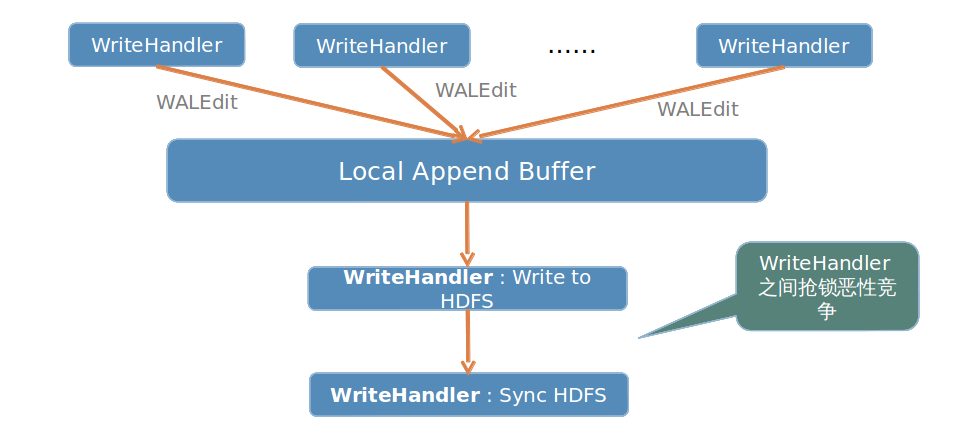
\includegraphics[width=\textwidth, height=5cm]{old-write-model.png}
\end{frame}

\begin{frame}{\subsecname}
	参见:JIRA HBASE-8755 \\
	单独的Write/Sync/Notify线程,消除锁竞争 \\
	\bigskip
	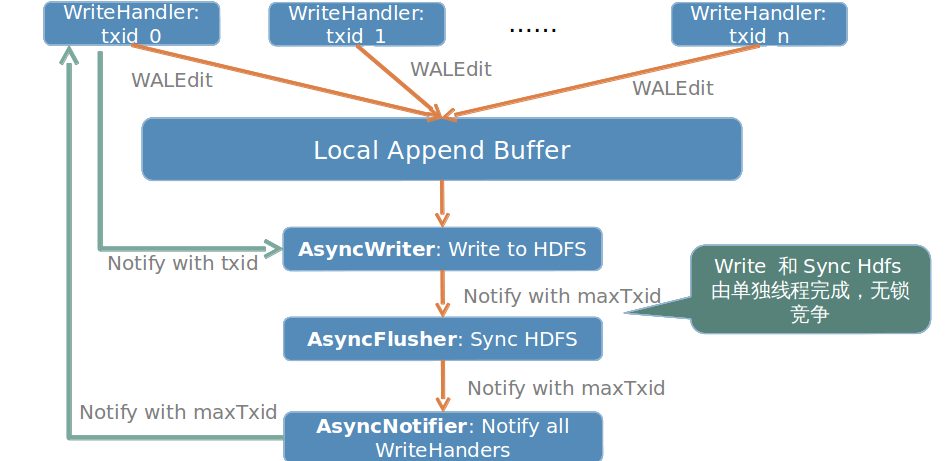
\includegraphics[width=\textwidth, height=5cm]{new-write-model.png}
\end{frame}

\begin{frame}{\subsecname}
	性能对比\\

	\bigskip
	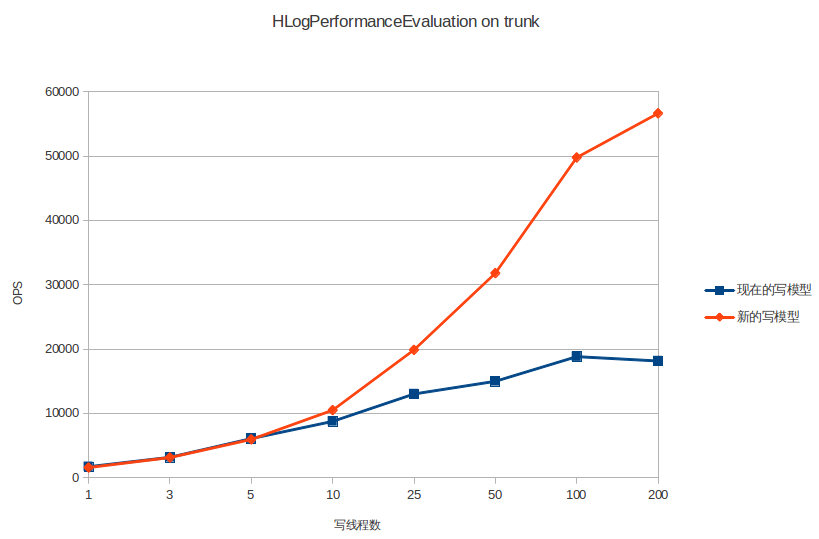
\includegraphics[width=\textwidth, height=5cm]{new-write-model-ops.png}
\end{frame}

\subsection{表/列族级别复制}
\begin{frame}{\subsecname}
	参见: jira HBASE-8751
	\begin{columns}
	\begin{column}{0.5\textwidth}
	add\_peer时指定表名和列族名 \\
	eg: add\_peer '1', peer\_addr, 'tableA:cf1'
	\end{column}
	\begin{column}{0.5\textwidth}
	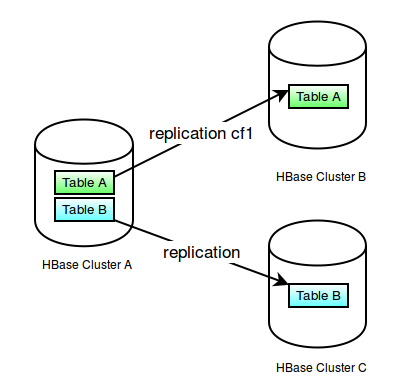
\includegraphics[width=\textwidth, height=4cm]{replication.png}
	\end{column}
\end{columns}
\end{frame}

\subsection{局部二级索引}
% local secondary index
\begin{frame}{\subsecname}
	\begin{enumerate}
		\item HBase只支持行Key上的的索引
		\item 其他的索引需要用户自己建
		\item 怎么保证数据和索引之间的一致性? \\
	\end{enumerate}
	\bigskip
\end{frame}

\begin{frame}{\subsecname}
 	场景: 用户为中心的数据, 只需要局部二级索引. \\

	\bigskip
	\begin{tabular}{|c|c|c|c|c|c|}
		\rowcolor{gray!50}
		\hline
		类型 & 行 & 列族 & 列 & 版本 & 值 \\
		\hline
		数据行 & UserId-xxx &  data &  c & ... &  value \\
		\rowcolor{green}
		\hline
		索引行 & UserId-value & c-index & ... & ... & UserId-xxx \\
		\hline
	\end{tabular}
	\\
	\bigskip
	\begin{itemize}
		\item 索引建立: 客户端建索引,将数据行和索引行作为一个批量写,写入HBase
		\item 查询: 先查询索引行获取数据行的Row Key, 在根据Row Key查询实际数据
	\end{itemize}
\end{frame}

\begin{frame}{\subsecname}
	怎么保证数据和索引一致性?
	\begin{itemize}
		\item \begin{block}{Region分割策略}
					前缀分割策略(KeyDelimiterPrefixRegionSplitPolicy) \\
					123123-34141 $\rightarrow$ 123123- \\
					保证同一个用户数据不会被分割在不同的region上
					\end{block}
		\item \begin{block}{Region内批量写的原子性}
					修改multi操作,对特定的表的multi操作,取到所有Row的行锁后才能继续,
					保证所有操作有相同的mvcc, 并且写在hlog里面在同一个记录里面。
					\end{block}
	\end{itemize}

	JIRA状态: 即将提交
\end{frame}

\subsection{名字服务}
% nameservie
\begin{frame}{\subsecname}
HBase集群的标识: \\
\bigskip
\textcolor{blue}{zkQuorum:zkClientPort:hbaseZnodeParent} \\

\bigskip

例如: bjsrv-test集群 \\
\bigskip
\textcolor{blue}{bjsrv.hadoop.srv:2181:/hbase/bjsrv-test}
\end{frame}

\begin{frame}{\subsecname}
扩展集群标识: \\

hbase://\${zkName}-\${hbaseName}:\${zkPort}

\begin{block}{映射规则}
  例如: hbase://bjsrv-test:2181/TestTable
	\begin{itemize}
	\item bjsrv $\rightarrow$ bjsrv.hadoop.srv
	\item 2181 $\rightarrow$ 2181, 默认是2181
	\item bjsrv-test $\rightarrow$ /hbase/bjsrv-test
	\end{itemize}
\end{block}

\begin{block}{使用}
  HTable table = new HTable(conf, "hbase://bjsrv-test/TestTable");
\end{block}

\begin{block}{优势}
  简化客户端配置,集群配置对业务透明
\end{block}
\end{frame}

\begin{frame}{\subsecname}
	其他支持
	\begin{itemize}
		\item \begin{block}{HBase Shell}
				\small eg: bin/hbase-cluster hbase://bjsrv-test shell
			\end{block}
		\item \begin{block}{Replication}
				\small eg: add\_peer '1', 'hbase://bjsrv-test', 'TestTable:CF'
			\end{block}
		\item \begin{block}{Mapreduce}
				\small eg: ./hbase CopyTable --peer.adr=hbase://bjsrv-test TestTable
			\end{block}
	\end{itemize}
	JIRA状态: 即将提交
\end{frame}

\section{未来开发计划}
\begin{frame}{开发计划}
\begin{itemize}
	\item 同步复制
	\item 跨行跨表的原子性(参考:Google Percolator)
	\item 全局二级索引
	\item Compaction优化. 参见: JIRA HBASE-9528
	\item Failover相关的优化. 参见:JIRA HBASE-9873
	\item 多租户共享集群与共有云
	\item HMaster重构. 参见:JIRA HBASE-5487
	\item ...
\end{itemize}
\end{frame}

\begin{frame}{与社区共同发展}
\begin{itemize}
	\item HBase修改反馈回社区(问题抽象/可配置)
	\item 紧跟社区最新进展 
	\item 积极参与社区方案设计和讨论 
\end{itemize}
\end{frame}

% Last slide
\begin{frame}[plain,c]
	\begin{center}
		\Huge 谢谢! 问题? \\
		\bigskip
		\bigskip
		\large
		邮箱: liushaohui@xiaomi.com\\ 
		微博: lshmouse
	\end{center}
\end{frame}

\end{CJK}
\end{document}
